\documentclass[a4paper,12pt]{article}
\usepackage{graphicx}
\usepackage{amsmath}
\usepackage{tkz-euclide}
\usepackage{booktabs}
\usepackage{multicol}
\title{Assignment-4\\ Latex Report}
\author{Fuzayil Bin Afzal Mir}
\date{25/01/2021} 

\begin{document}
\begin{multicols}{2}
	\maketitle
	
	
	\newpage
	\begin{itemize}
	    \item \Large\textbf{Exercise 2.9}
	\end{itemize}
	\section{Draw a $\triangle$ABC, given that a+b+c=
	11, $\angle$B = 30$^{\circ}$ and $\angle$C = 90$^{\circ}$}\\
\subsection{Solution} \\

\textbf{Figure of triangle ABC}

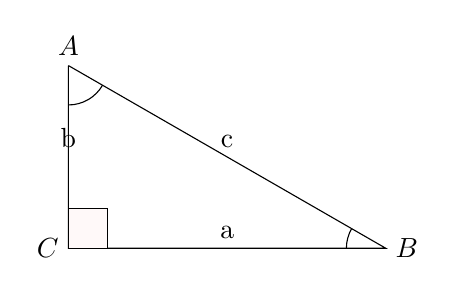
\begin{tikzpicture}[scale=1]
    \coordinate[label=right:$B$] (B) at (4.03,0);
    \coordinate[label=left:$C$] (C) at (0,0);
    \coordinate[label=above:$A$] (A) at (0,2.32);
    
    \draw (A)--node[above] {$\textrm{c}$}
    (B)--node[above] {$\textrm{a}$}
    (C)--node[above] {$\textrm{b}$}(A);
    \tkzMarkAngle[fill=green!15,size=0.5](C,A,B);
    
    \tkzMarkRightAngle[fill=pink!10,size=0.5](B,C,A);
    
     \tkzMarkAngle[fill=green!30,size=0.5](A,B,C);
    \end{tikzpicture}





It,s given that, \begin{equation}
    a+b+c=11
\end{equation}
\\

Using sin rule we get\\

\dfrac{sinA}{a}=\dfrac{sinB}{b}=\dfrac{sinC}{c}\\

Using, \dfrac{sinB}{b}=\dfrac{sinC}{c}\\
       we get,\\
       
  \begin{equation}
    (0)a+2b-c=0
\end{equation}\\

\setlength{\columnsep}{1.5cm}
\setlength{\columnseprule}{0.2pt}
Also,\\
 Cos(30$^{\circ}$ )= \dfrac{a}{c}\\
       we get,\\
       
   
  \begin{equation}
    2a+0b-\sqrt{3}(c)=0
\end{equation}
Writing Equations (1),(2) and (3) in matrix form,\\

\begin{pmatrix}
		1 & 1 & 1\\
		0 & 2 & -1\\ 
		2 & 0 & -\sqrt{3}\\
	\end{pmatrix}\begin{pmatrix}
		 a\\
		 b\\
		 c\\
    	\end{pmatrix} = \begin{pmatrix}
		 11\\
		 0\\
		 0\\
    	\end{pmatrix}\\

By using elementary row operations, we get\\

\fbox{a=\dfrac{403}{100}}\\

\fbox{b=\dfrac{232}{100}}\\

\fbox{ c=\dfrac{465}{100}}\\
\end{multicols}

\newpage


\subsection{Figure of $\triangle$ABC,}
\begin{figure}[htp]
    \centering
    \includegraphics[width=10cm]{triangle.jpg}
    \caption{Fig generated using python}
    \label{fig:2}
\end{figure}
 \\
 
 \textbf{Download the python code used for generating the figure from here:}
 
 \fbox{
 \begin{lstlisting}
 https://github.com/FuzayilMir/Assignment-4-Construct/blob/main/TRICODE.py
 \end{lstlisting}
}






















\end{document}